The purpose of the functions related to the query language is to work with huge
BioPAX files and extract from the BioPAX documents only the information that is
of interest. For this part, we will use the apoptosis example initially
extracted from Reactome database: Apoptosis3.owl (extracted from the Reactome
database, available from our website). This set of functions can be used with
big pathway databases already exported to BioPAX, such as Reactome, BioCyc,
NetPath (see \url{http://www.biopax.org} for the complete list).

\subsection{Generate Index}
\textbf{Plugins$\Rightarrow$BiNoM 2.0$\Rightarrow$BiNoM BioPAX 3 Query$\Rightarrow$Generate Index}\\

Using this function BiNoM maps the content of BioPAX file onto a labeled graph
(referred to as index). It creates an *.xgmml file from an *.owl one
(figure~\ref{Generate_BioPAX_Index}). For the definition of BioPAX index, see
section~\ref{Standard_BioPAX_Interfaces}.

\begin{figure}
\centering
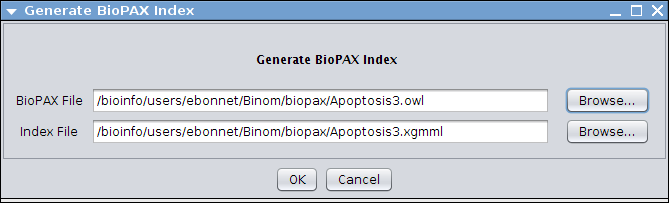
\includegraphics[width=0.8\textwidth]{graphics/ebo_generate_BioPAX_Index}
\caption{Dialog for generating a BioPAX Index.}
\label{Generate_BioPAX_Index}
\end{figure}

\subsection{Load Index}
\textbf{Plugins$\Rightarrow$BiNoM 2.0$\Rightarrow$BiNoM BioPAX 3 Query$\Rightarrow$Load Index}\\

Once the xgmml is created, it can be loaded into memory. The index is a global
object, i.e. only one index can be used at a time. The function ``Load Index`` loads the index
file from xgmml format (figure~\ref{Load_Index_Dialog}).\\\\

\begin{figure}
\centering
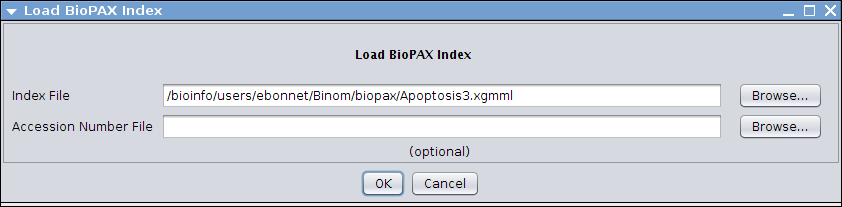
\includegraphics[width=0.8\textwidth]{graphics/ebo_load_BioPAX_Index}
\caption{Load Index dialog.}
\label{Load_Index_Dialog}
\end{figure}

Together with the index, you can also upload a tab-delimited “accession number
file” which corresponds to a list of synonyms for the genes/proteins ids used in
a network (see an example of the content of some accession number file at
figure~\ref{Accession_Number_File}). An entity in the index can be identified by
its id, by any XREF attribute (see section~\ref{Standard_BioPAX_Interfaces}), by
node name, or by any synonym from the accession table (if it is provided).

\begin{figure}
\centering
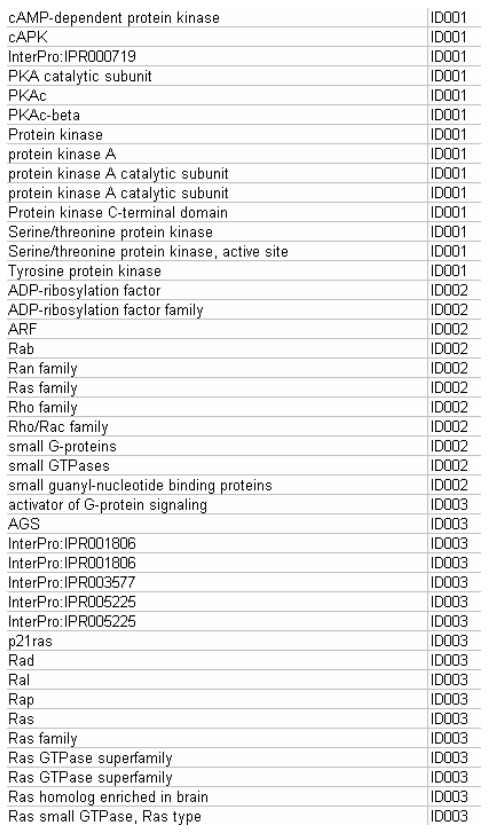
\includegraphics[width=8 cm]{graphics/Accession_Number_File}
\caption{Example of accession Number file. First column is a synonym (which can have structure $\textless database\textgreater :\textless standard_id\textgreater)$, the second column is the id used inside the BioPAX file.}
\label{Accession_Number_File}
\end{figure}

\subsection{Display Index Info}
\textbf{Plugins$\Rightarrow$BiNoM 2.0$\Rightarrow$BiNoM BioPAX 3 Query$\Rightarrow$Display Index Info}\\

This command opens a window indicating the name of the graph, the name of the
file, the accession number file, when available, the number of records, and the
various statistics of the index: number of publications, proteins,
physicalEntities, complexes, biochemical reactions, pathways, pathwaySteps,
catalyses, and modulations (necessary proteins for catalyses). See
figure~\ref{BioPAX_Index_Info}.

\begin{figure}[h]
\centering
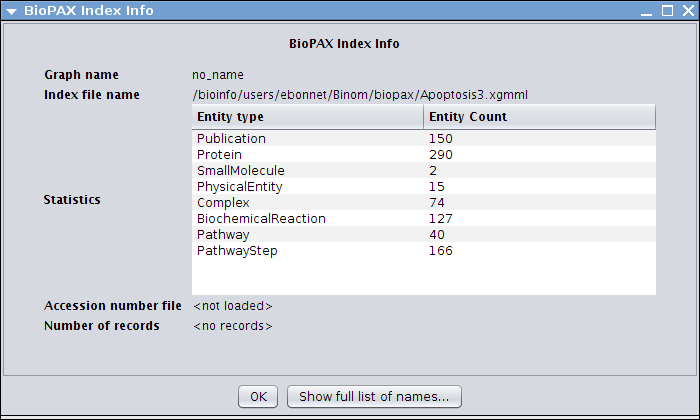
\includegraphics[width=0.8\textwidth]{graphics/ebo_biopax_index_info}
\caption{Display Index info.}
\label{BioPAX_Index_Info}
\end{figure}

\subsection{Select Entities}
\textbf{Plugins$\Rightarrow$BiNoM 2.0$\Rightarrow$BiNoM BioPAX 3 Query$\Rightarrow$Select Entities}\\

The BioPAX document is often too big to find the protein or gene that needs to
be studied. To access it easily and rapidly, it is possible to find the
component directly with this command and build a specific network around that
molecule.\\\\
For example, in the Apoptosis3 network, we choose to find the SMAC protein and extend the
network around it. A dialog window pops up and offers the possibility to
find a protein or a gene by its name or id or XREF attribute or synonym, from
the current network when a network is already opened, or from the list of
identities associated with the BioPAX index
(figure~\ref{Select_entities_from_index}).\\\\

For our example, we choose the second option. Note that it is possible to type
several versions of the protein name (separated by space, comma, or semi-colon
symbols). A new network is created, having only one node (SMAC). It is also
possible to select more than one entity, in this case, the components all appear
in the same window.\\\\

It is also an option to view several genes or proteins in the same network by
checking “output in the current network”.\\\\

\begin{figure}
\centering
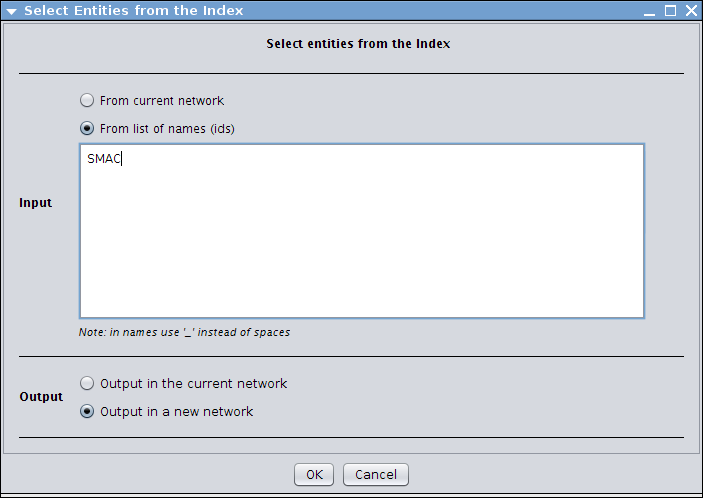
\includegraphics[width=0.8\textwidth]{graphics/ebo_select_entities_from_the_index}
\caption{Select entities from the index.}
\label{Select_entities_from_index}
\end{figure}

Note that it is advised to use the BiNoM BioPAX visual style to view the resulting network.

\subsection{Standard Query}
\textbf{Plugins$\Rightarrow$BiNoM 2.0$\Rightarrow$BiNoM BioPAX 3 Query$\Rightarrow$Standard Query}\\

This command proceeds through a series of actions that will extend the initial
network.\\\\
Let’s start with diverse queries from the network created from the Apoptosis
file with the initial SMAC entity. A dialog window opens as
figure~\ref{Standard_Query_Dialog}.\\\\

\begin{figure}
\centering
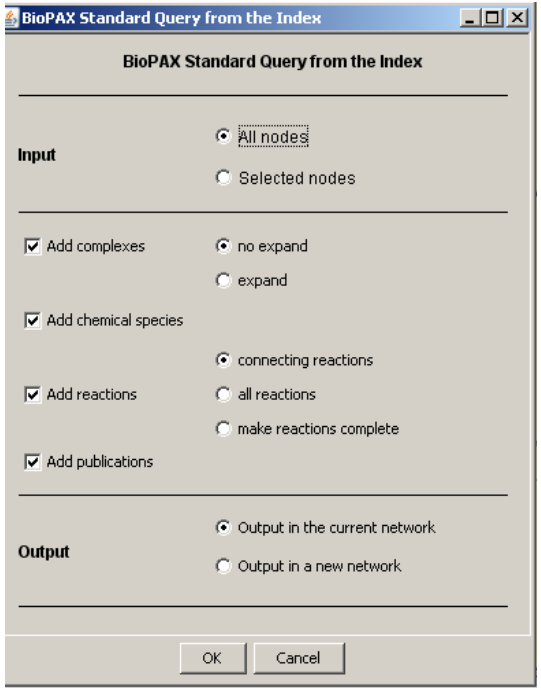
\includegraphics[width=.5\textwidth]{graphics/Standard_Query_Dialog}
\caption{BioPAX Standard Query: dialog window.}
\label{Standard_Query_Dialog}
\end{figure}

All the options proposed in the dialog window (figure~\ref{Standard_Query_Dialog}) are listed here:

\subsubsection{Input}

In the network, you can submit queries that concern all the nodes (option All Nodes) in the network or only the selected nodes (option Selected nodes). 

\subsubsection{Adding nodes}


\begin{itemize}
\item Add complexes
\begin{itemize}
\item The option “no expand” adds only the homodimers of the molecule. If several proteins were queried,
then all hetero-dimers in which all the proteins participate would be selected.
\item The option “expand” adds all the complexes in which SMAC is involved
(figure~\ref{Standard_Query_Add_complexes}b). The green arrow with a diamond
ending represents the inclusion of one protein in a complex form.
\end{itemize}

\begin{figure}
\centering
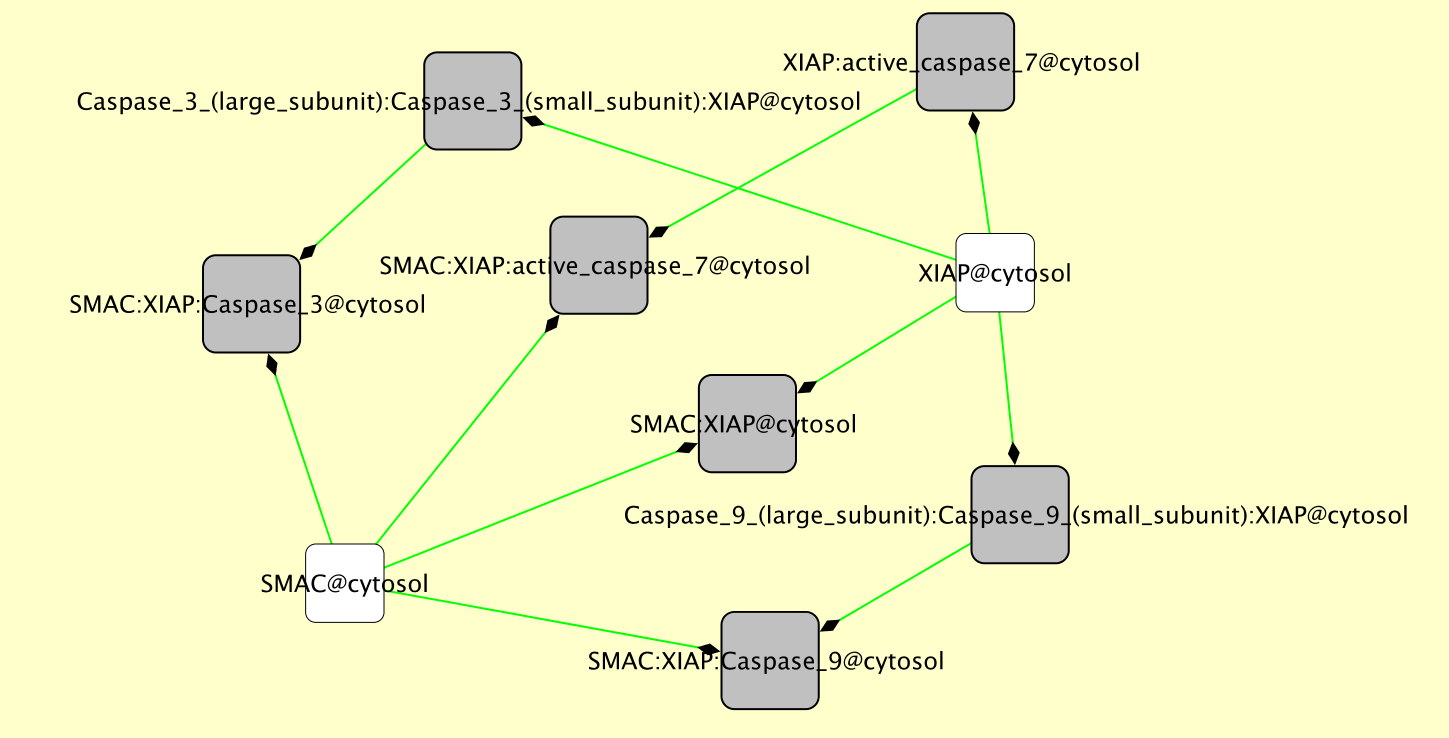
\includegraphics[width=0.8\textwidth]{graphics/ebo_smac_prot_complex}
\caption{BioPAX Standard Query: Complexes involving SMAC are added to the network.}
\label{Standard_Query_Add_complexes}
\end{figure}

\item Add chemical species\\
This function adds, for each species, the cellular location and its specified modifications.

%\begin{figure}
%\centering
%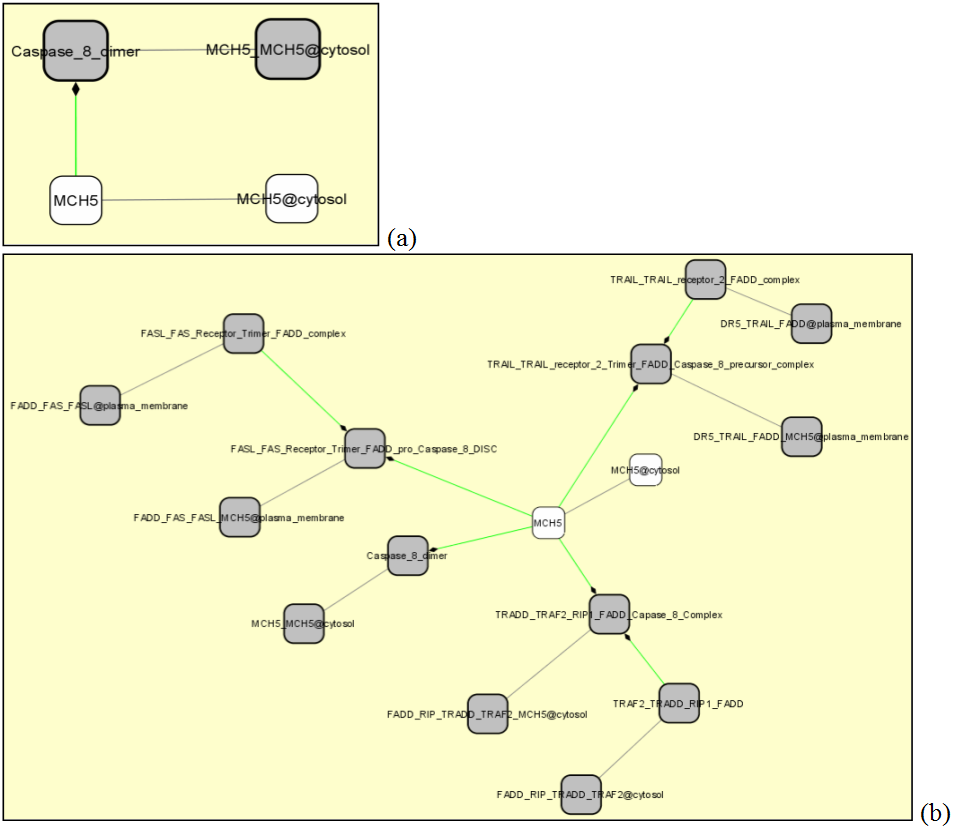
\includegraphics[width=0.8\textwidth]{graphics/Standard_Query_Chemical_species}
%\caption{Chemical species. Cellular locations of all forms of MCH5.}
%\label{Standard_Query_Chemical_species}
%\end{figure}

\item Add reactions
\begin{itemize}
\item The option ''connecting reactions'' connects all present species that have common reactions (Figure~\ref{Standard_Query_All_connecting_reactions}).

\begin{figure}
\centering
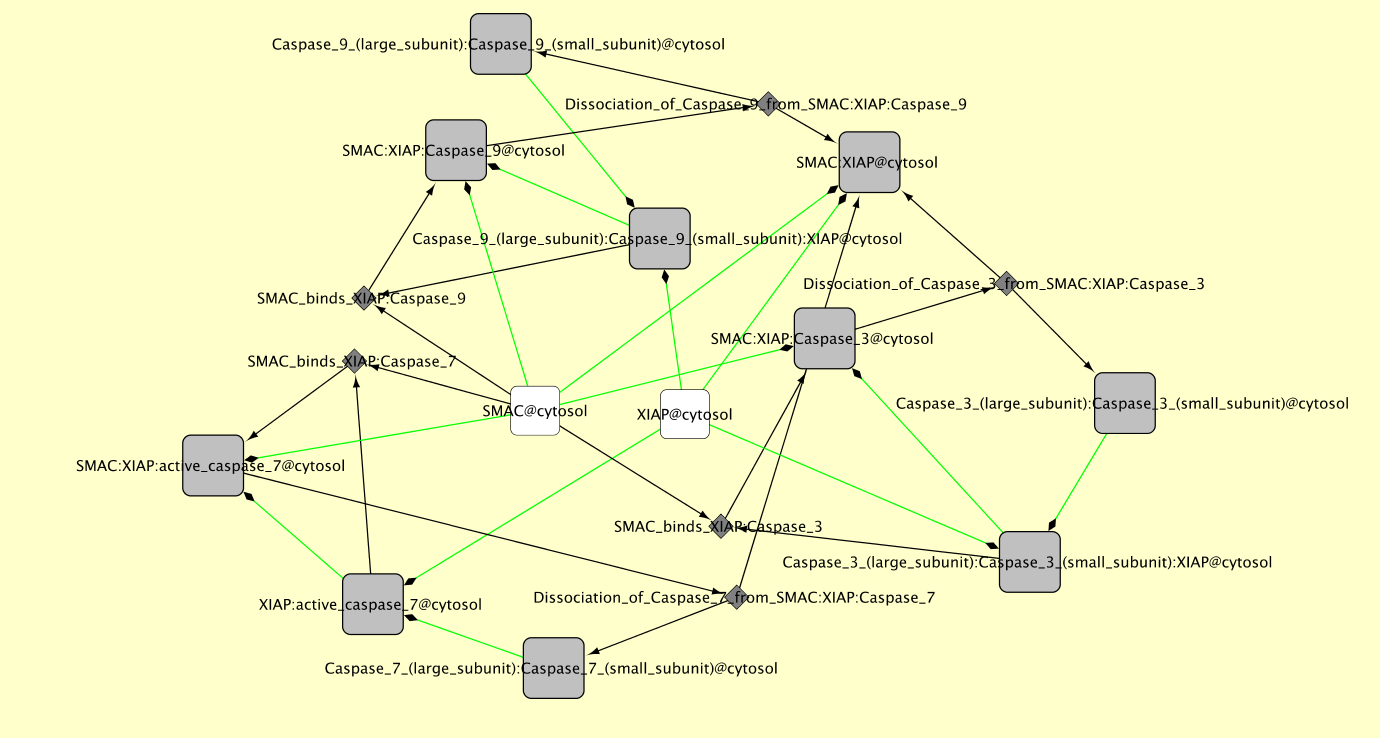
\includegraphics[width=0.8\textwidth]{graphics/ebo_smac_add_reactions}
\caption{Adding reactions: SMAC centered network expanded with the connecting reactions.}
\label{Standard_Query_All_connecting_reactions}
\end{figure}

\item The option ``all reactions`` includes all the reactions involving the chemical species.

%\begin{figure}
%\centering
%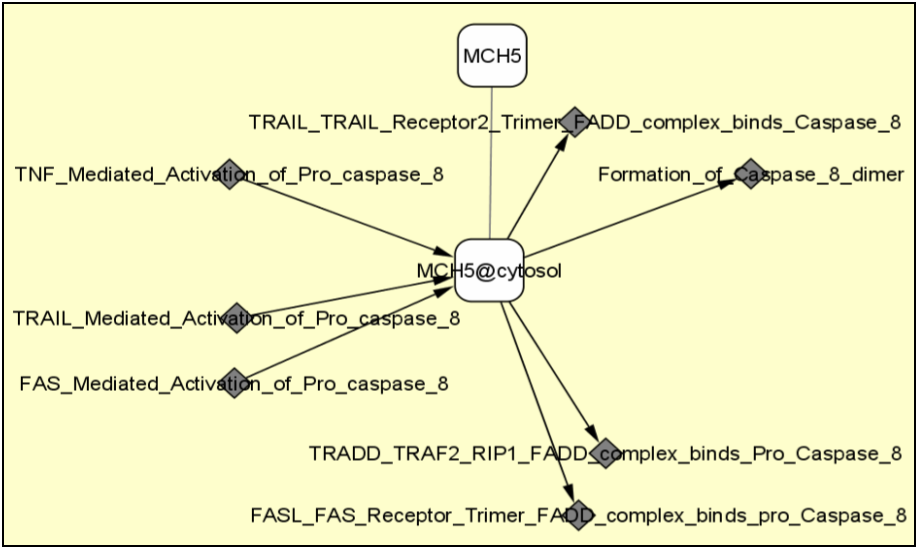
\includegraphics[width=0.8\textwidth]{graphics/Standard_Query_Adding_all_reactions}
%\caption{Adding reactions: example adding all reactions.}
%\label{Standard_Query_Adding_all_reactions}
%\end{figure}

\item The option ''make reactions complete'' adds all the sources and targets of the
reactions listed in the BioPAX index, including the pathway nodes and publications links.

%\begin{figure}
%\centering
%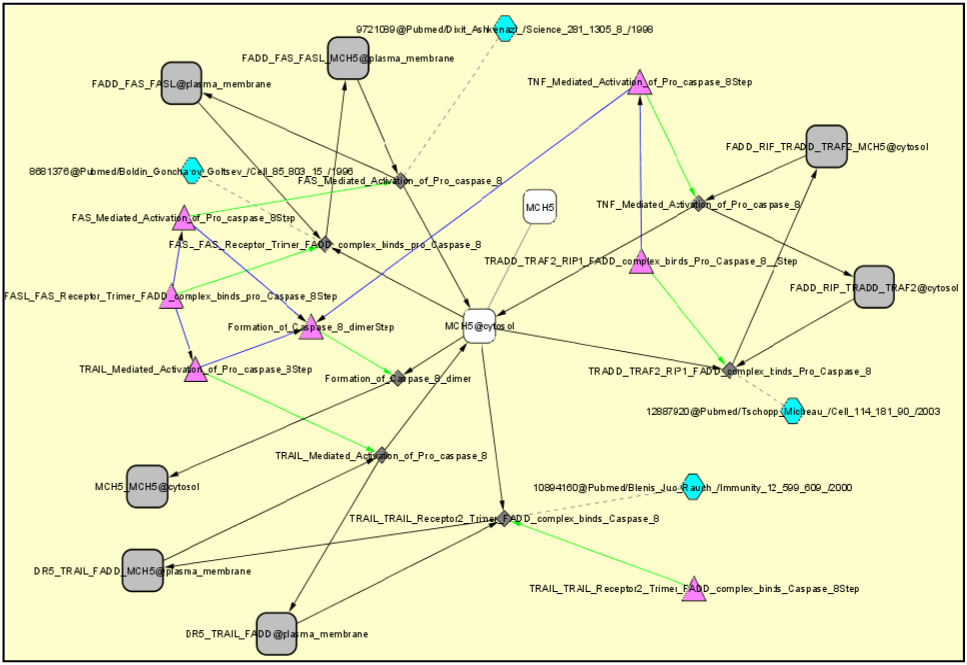
\includegraphics[width=0.8\textwidth]{graphics/Standard_Query_Making_reactions_complete}
%\caption{Adding reactions: example when making the reactions complete.}
%\label{Standard_Query_Making_reactions_complete}
%\end{figure}

\end{itemize}
\item Add publications\\
When available, this function adds all the references associated with a reaction (see figure~\ref{Standard_Query_Adding_publications}).

\begin{figure}
\centering
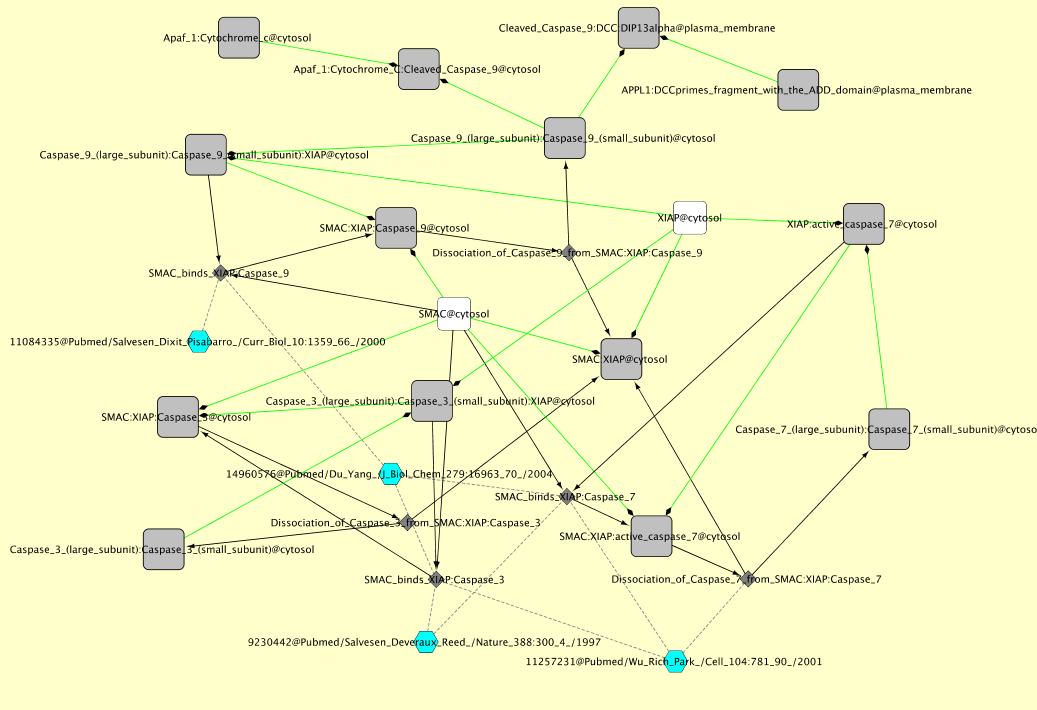
\includegraphics[width=0.8\textwidth]{graphics/ebo_smac_publications}
\caption{Adding publications.}
\label{Standard_Query_Adding_publications}
\end{figure}

\end{itemize}

\subsubsection{Output}
The result of the queries can be seen either in the current network or in a new network.

\parbox{\textwidth}{

\subsection{Index Path Analysis}

\textbf{Plugins$\Rightarrow$BiNoM 2.0$\Rightarrow$BiNoM BioPAX 3 Query$\Rightarrow$Index Path Analysis}\\

This command finds the directed or non-directed, shortest, optimal or
suboptimal, non intersecting paths with a pre-defined number of intermediaries
in an index file. Note that the species need to be selected on a graph before
this query.\\\\
This part of the query engine uses the same algorithms and options as Path
analysis dialog (see section~\ref{Path_Analysis}), however, with the network
(index) kept completely in memory, without explicit visualization. Moreover, the
network is slightly modified before this type of query: in particular, all
non-directed edges (of CONTAINS, SPECIESOF and some other types) are represented
as bi-directional, some nodes (publications and, optionally, smallMolecules) are
removed.\\\\
For example, the following steps

\begin{enumerate}
\item Select Entities: specify SMAC and XIAP proteins.
\item Select the two nodes.
\item Index Path analysis: Find all non-intersecting paths.
\item BiNoM Analysis: Extract Reaction Network.
\end{enumerate}

will produce the following network connecting SMAC and XIAP proteins (Figure~\ref{Index_Path_Analysis}).

}

\begin{figure}
\centering
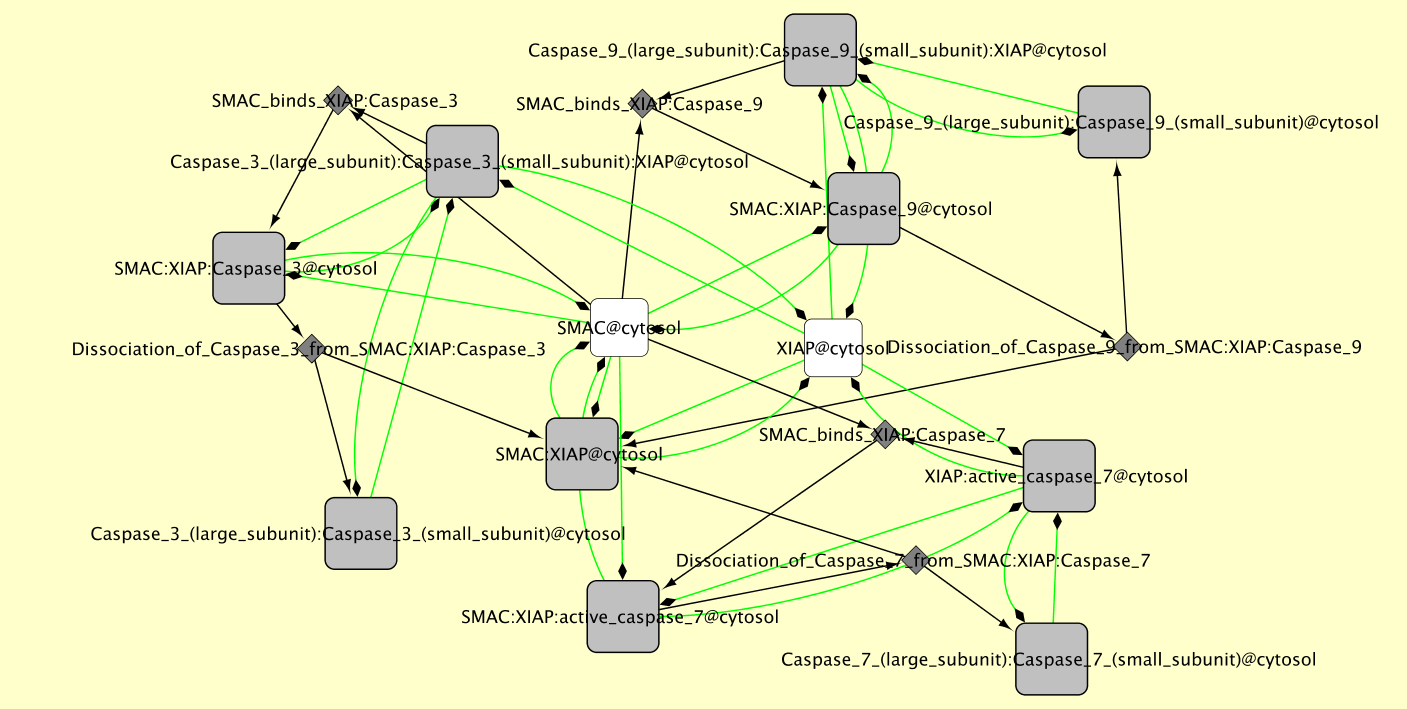
\includegraphics[width=0.8\textwidth]{graphics/ebo_index_path}
\caption{Index path Analysis with SMAC and XIAP.}
\label{Index_Path_Analysis}
\end{figure}

\subsection{View Query Log}
\textbf{Plugins$\Rightarrow$BiNoM 2.0$\Rightarrow$BiNoM BioPAX 3 Query$\Rightarrow$View Query Log}\\
In this window are recapitulated all the queries done during the session.

%\begin{figure}[h]
%\centering
%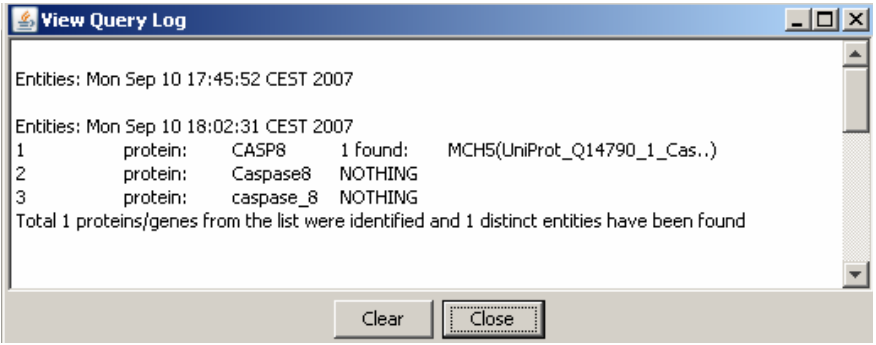
\includegraphics[width=0.8\textwidth]{graphics/BioPAXViewQueryLogDialog}
%\caption{View Query Log Dialog}
%\label{BioPAXViewQueryLogDialog}
%\end{figure}